\documentclass[11pt, a4paper]{article}
\usepackage{pdfpages}
\usepackage{parallel}
\usepackage[T2A]{fontenc}
\usepackage{ucs}
\usepackage[utf8x]{inputenc}
\usepackage[polish,english,russian]{babel}
\usepackage{hyperref}
\usepackage{rotating}
\usepackage[inner=2cm,top=1.8cm,outer=2cm,bottom=2.3cm,nohead]{geometry}
\usepackage{listings}
\usepackage{graphicx}
\usepackage{wrapfig}
\usepackage{longtable}
\usepackage{indentfirst}
\usepackage{array}
\usepackage{tikzsymbols}
\usepackage{soul}
\usepackage[ruled,vlined]{algorithm2e}
%\counterwithout{figure}{section} 

\usepackage{url}
\makeatletter
\g@addto@macro{\UrlBreaks}{\UrlOrds}
\makeatother

\newcolumntype{P}[1]{>{\raggedright\arraybackslash}p{#1}}
\frenchspacing
\usepackage{fixltx2e} %text sub- and superscripts
\usepackage{icomma} % коскі ў матэматычным рэжыме
\PreloadUnicodePage{4}

\newcommand{\longpage}{\enlargethispage{\baselineskip}}
\newcommand{\shortpage}{\enlargethispage{-\baselineskip}}

\def\switchlang#1{\expandafter\csname switchlang#1\endcsname}
\def\switchlangbe{
\let\saverefname=\refname%
\def\refname{Літаратура}%
\def\figurename{Іл.}%
}
\def\switchlangen{
\let\saverefname=\refname%
\def\refname{References}%
\def\figurename{Fig.}%
}
\def\switchlangru{
\let\saverefname=\refname%
\let\savefigurename=\figurename%
\def\refname{Литература}%
\def\figurename{Рис.}%
}

\hyphenation{admi-ni-stra-tive}
\hyphenation{ex-pe-ri-ence}
\hyphenation{fle-xi-bi-li-ty}
\hyphenation{Py-thon}
\hyphenation{ma-the-ma-ti-cal}
\hyphenation{re-ported}
\hyphenation{imp-le-menta-tions}
\hyphenation{pro-vides}
\hyphenation{en-gi-neering}
\hyphenation{com-pa-ti-bi-li-ty}
\hyphenation{im-pos-sible}
\hyphenation{desk-top}
\hyphenation{elec-tro-nic}
\hyphenation{com-pa-ny}
\hyphenation{de-ve-lop-ment}
\hyphenation{de-ve-loping}
\hyphenation{de-ve-lop}
\hyphenation{da-ta-ba-se}
\hyphenation{plat-forms}
\hyphenation{or-ga-ni-za-tion}
\hyphenation{pro-gramming}
\hyphenation{in-stru-ments}
\hyphenation{Li-nux}
\hyphenation{sour-ce}
\hyphenation{en-vi-ron-ment}
\hyphenation{Te-le-pathy}
\hyphenation{Li-nux-ov-ka}
\hyphenation{Open-BSD}
\hyphenation{Free-BSD}
\hyphenation{men-ti-on-ed}
\hyphenation{app-li-ca-tion}

\def\progref!#1!{\texttt{#1}}
\renewcommand{\arraystretch}{2} %Іначай формулы ў матрыцы зліпаюцца з лініямі
\usepackage{array}

\def\interview #1 (#2), #3, #4, #5\par{

\section[#1, #3, #4]{#1 -- #3, #4}
\def\qname{LVEE}
\def\aname{#1}
\def\q ##1\par{{\noindent \bf \qname: ##1 }\par}
\def\a{{\noindent \bf \aname: } \def\qname{L}\def\aname{#2}}
}

\def\interview* #1 (#2), #3, #4, #5\par{

\section*{#1\\{\small\rm #3, #4. #5}}
\ifx\ParallelWhichBox\undefined%
    \addcontentsline{toc}{section}{#1, #3, #4}%
\else%
\ifnum\ParallelWhichBox=0%
    \addcontentsline{toc}{section}{#1, #3, #4}%
\fi\fi%

\def\qname{LVEE}
\def\aname{#1}
\def\q ##1\par{{\noindent \bf \qname: ##1 }\par}
\def\a{{\noindent \bf \aname: } \def\qname{L}\def\aname{#2}}
}

\newcommand{\interviewfooter}[1]{
\vskip 1em
\noindent \textit{#1}
}

\switchlang{en}
\begin{document}

\title{1987 "--- IBM PS/2 mouse}
\date{}
\maketitle
\selectlanguage{english}
This mouse, released in 1987, was the first to implement the PS/2 interface, which is still used in a number of desktop computers to connect keyboards and mice using a 6-pin mini-DIN connector.

\begin{figure}[h]
    \centering
    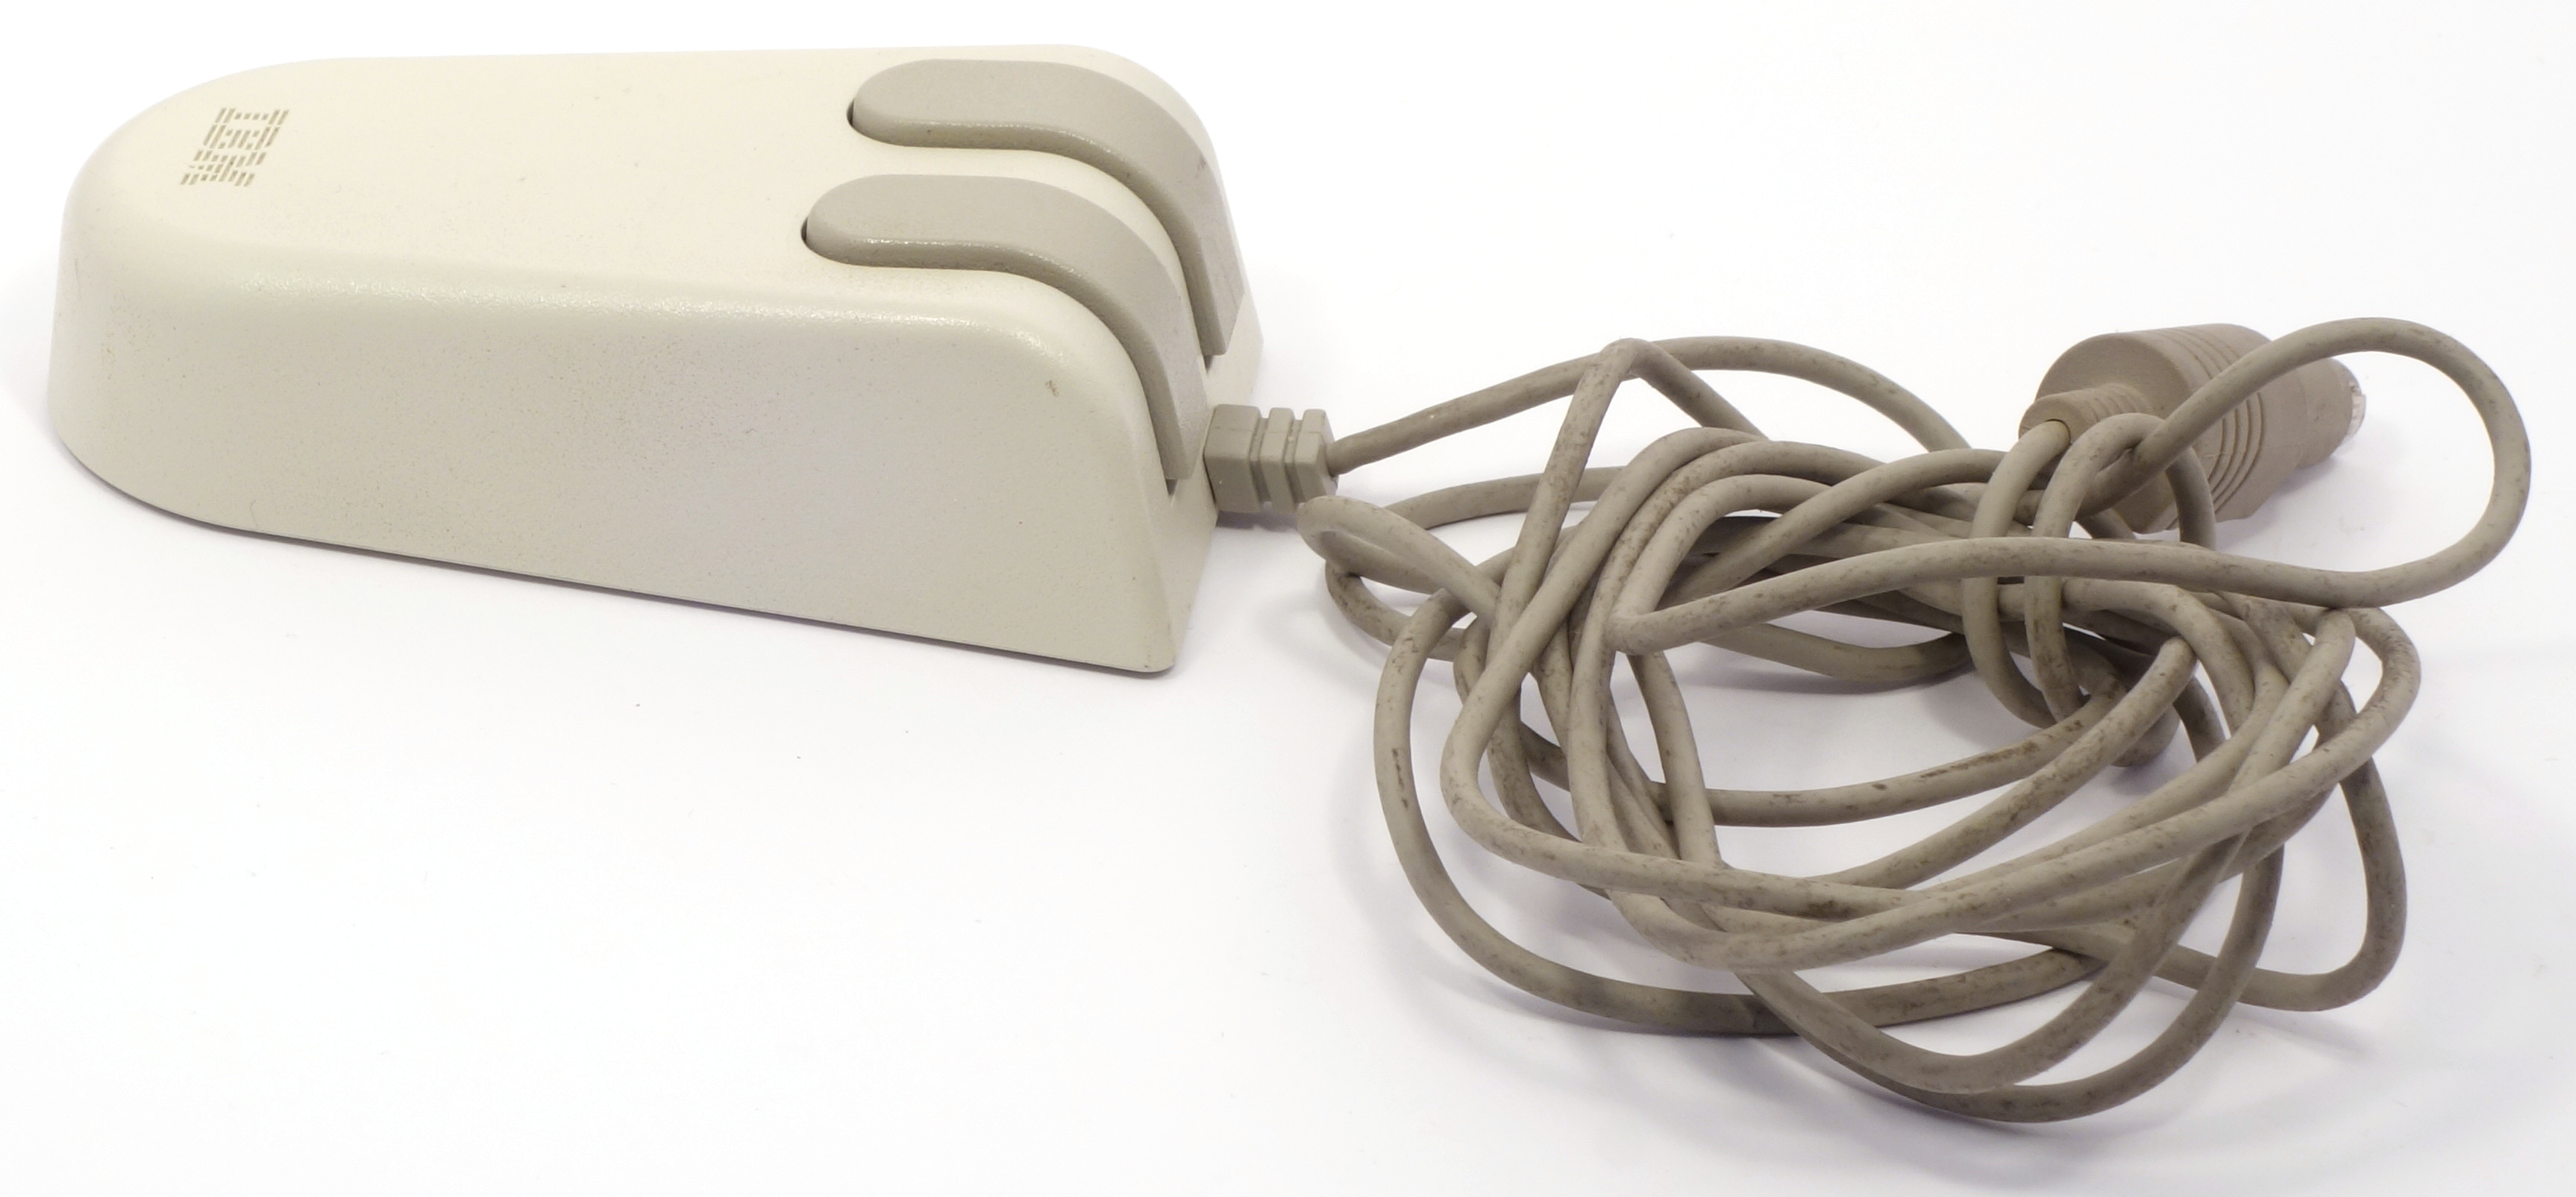
\includegraphics[scale=0.6]{1987_ibm_ps2_mouse/num0.JPG}
    \caption{IBM PS/2 Mouse}
    \label{fig:IMBPS2Pic}
\end{figure}

The first mouse with this interface was this device from IBM, available at relatively consumer prices in the late 80s. As you can see (figure \ref{fig:IMBPS2TopBottom}), there are two mechanical buttons and an embossed company logo on the top side of the case; in general, the case is minimalistic and, apart from that, does not contain any additional elements. The bottom contains the ball, and the two arrows on the ball's locking ring show the direction to unlock so it can be removed for cleaning the mouse.

\begin{figure}[h]
    \centering
    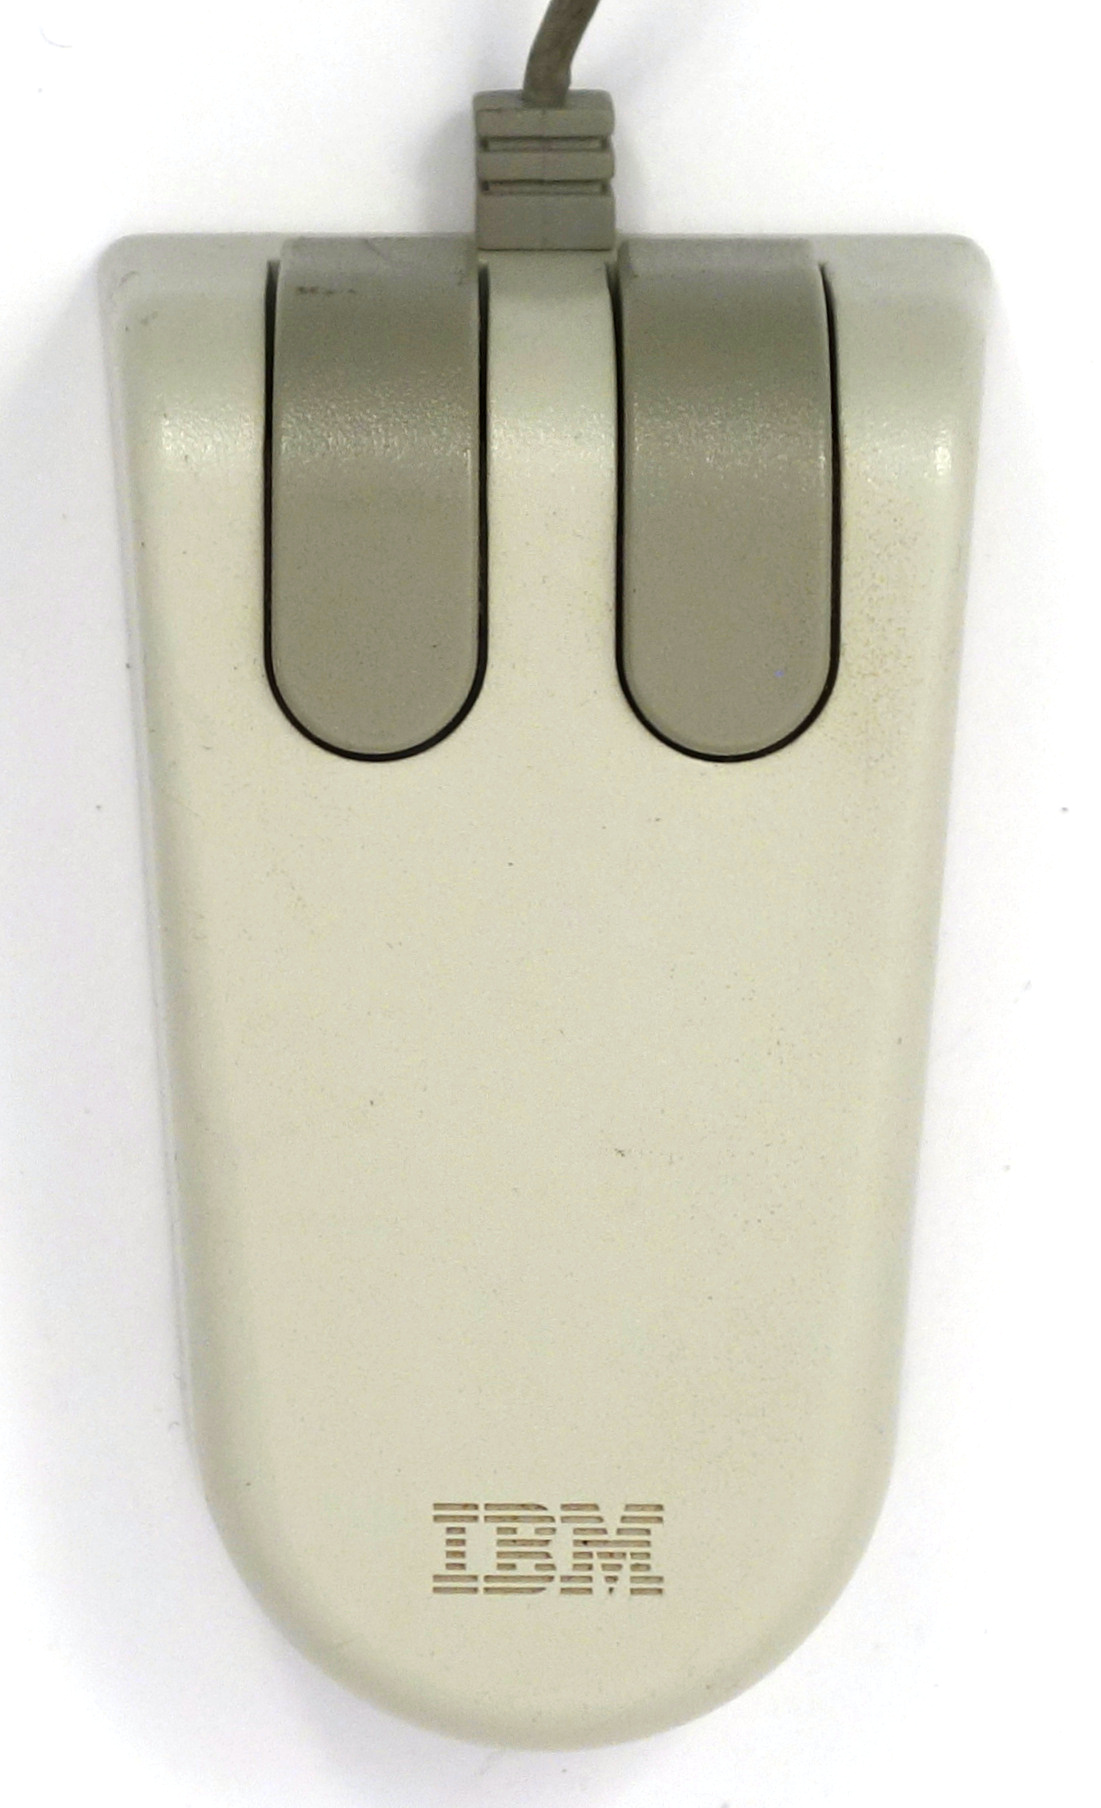
\includegraphics[scale=0.5]{1987_ibm_ps2_mouse/num1.JPG}
    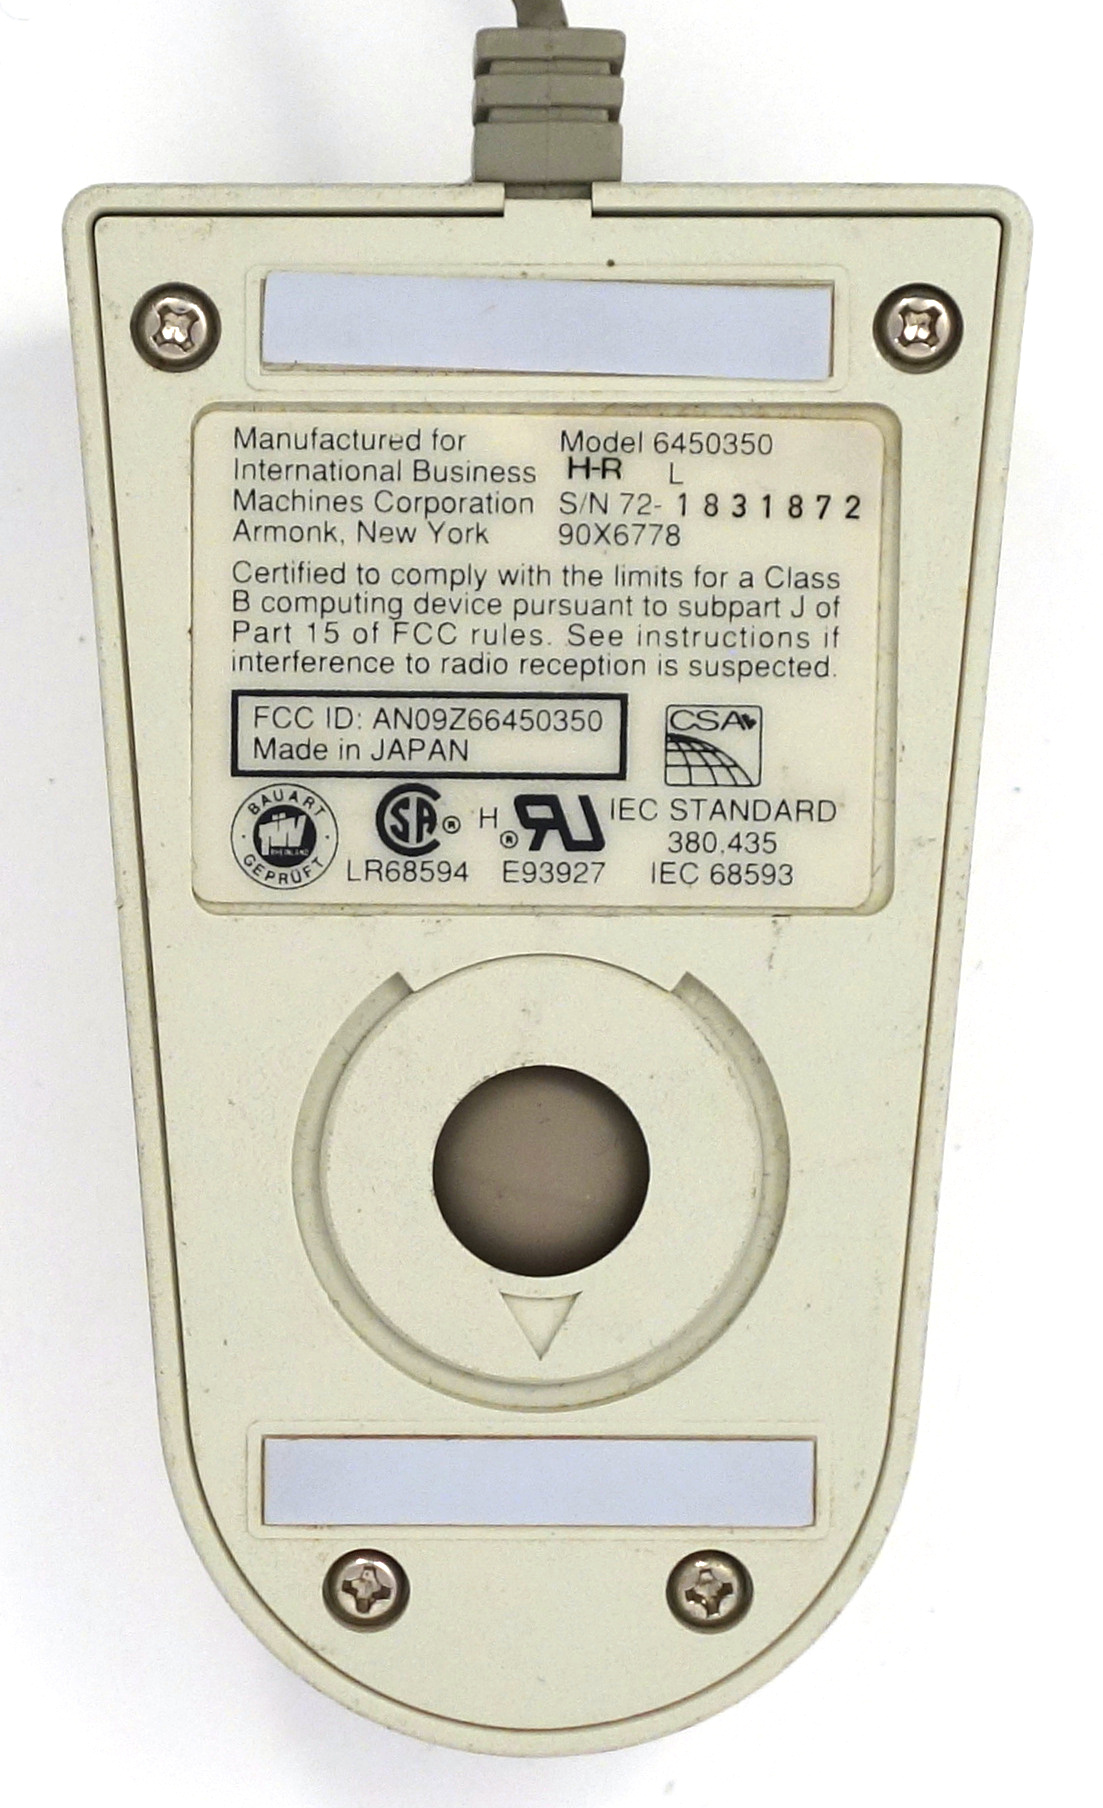
\includegraphics[scale=0.5]{1987_ibm_ps2_mouse/num2.JPG}
    \caption{IBM PS/2 Mouse, top and bottom views}
    \label{fig:IMBPS2TopBottom}
\end{figure}

\begin{figure}[h]
    \centering
    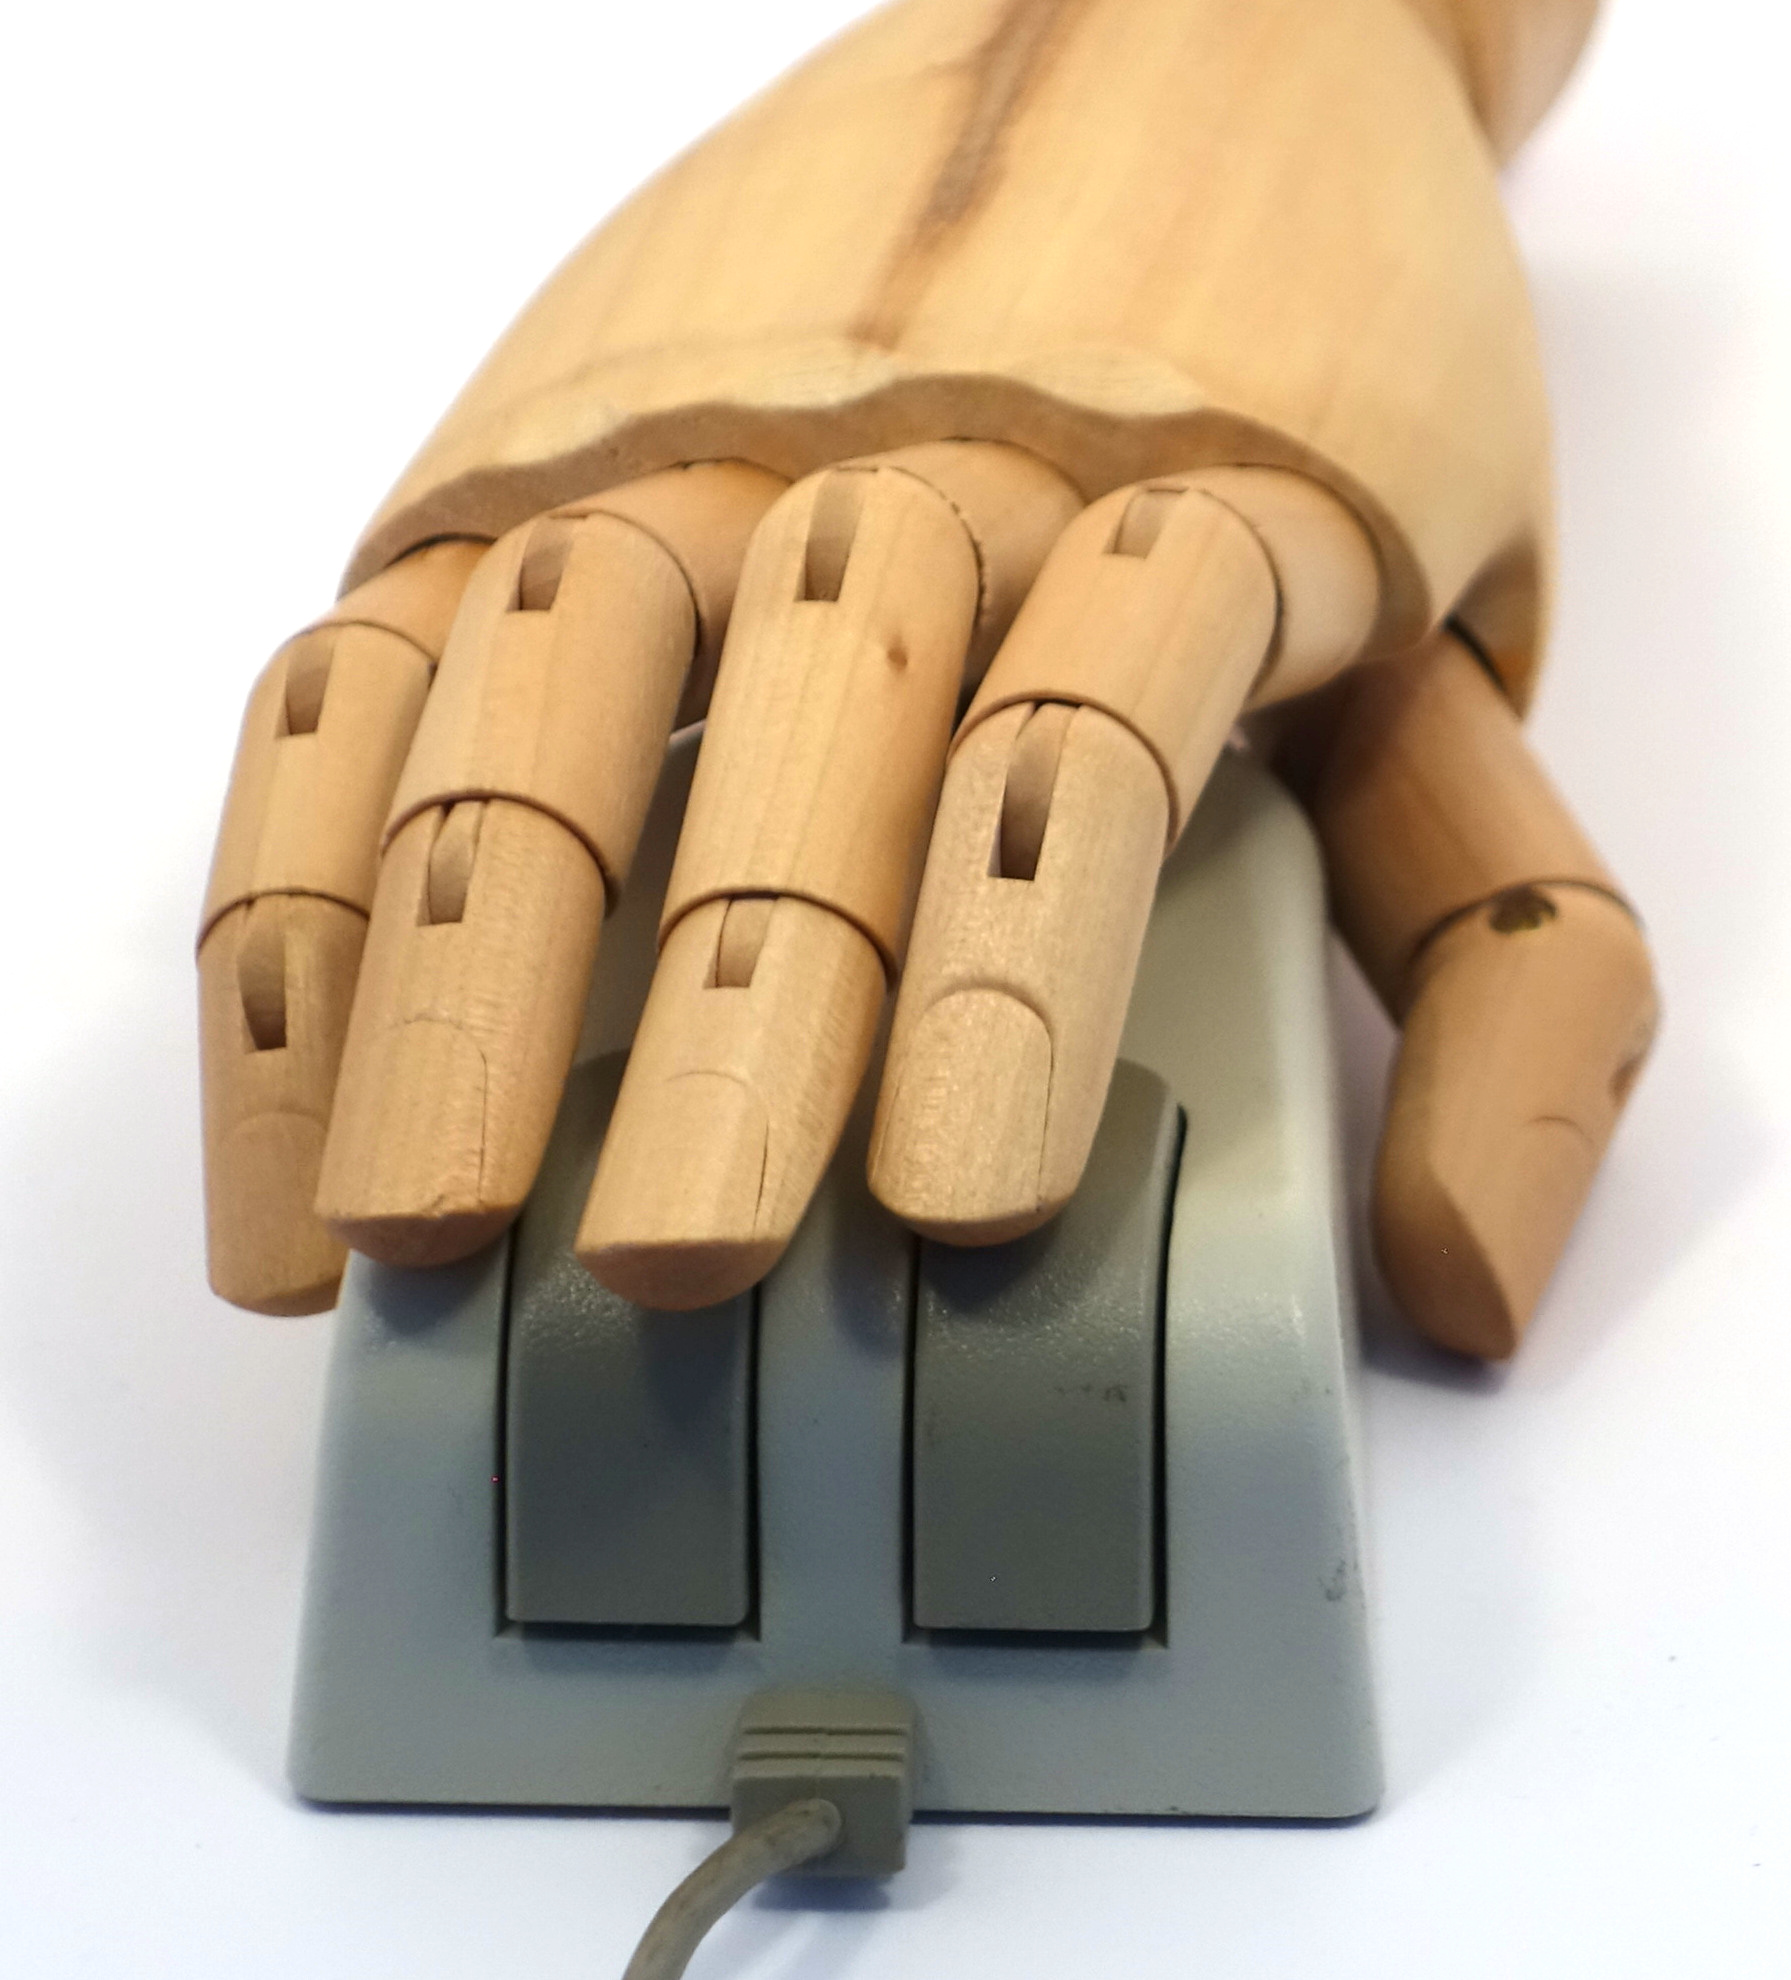
\includegraphics[scale=0.4]{1987_ibm_ps2_mouse/num3.JPG}
    \caption{IBM PS/2 Mouse with a human hand model}
    \label{fig:IMBPS2Hand}
\end{figure}

As you can see in figure \ref{fig:IMBPS2Hand}, the trapezoidal shape of the case allows you to wrap your fingers comfortably around the mouse and press the buttons in the natural position of the hand; however, the small size of the mouse (figure \ref{fig:IBMPS2Size}) does not allow the palm of the hand to rest on the body of the mouse, which puts additional strain on the wrist.

\begin{figure}[h]
    \centering
    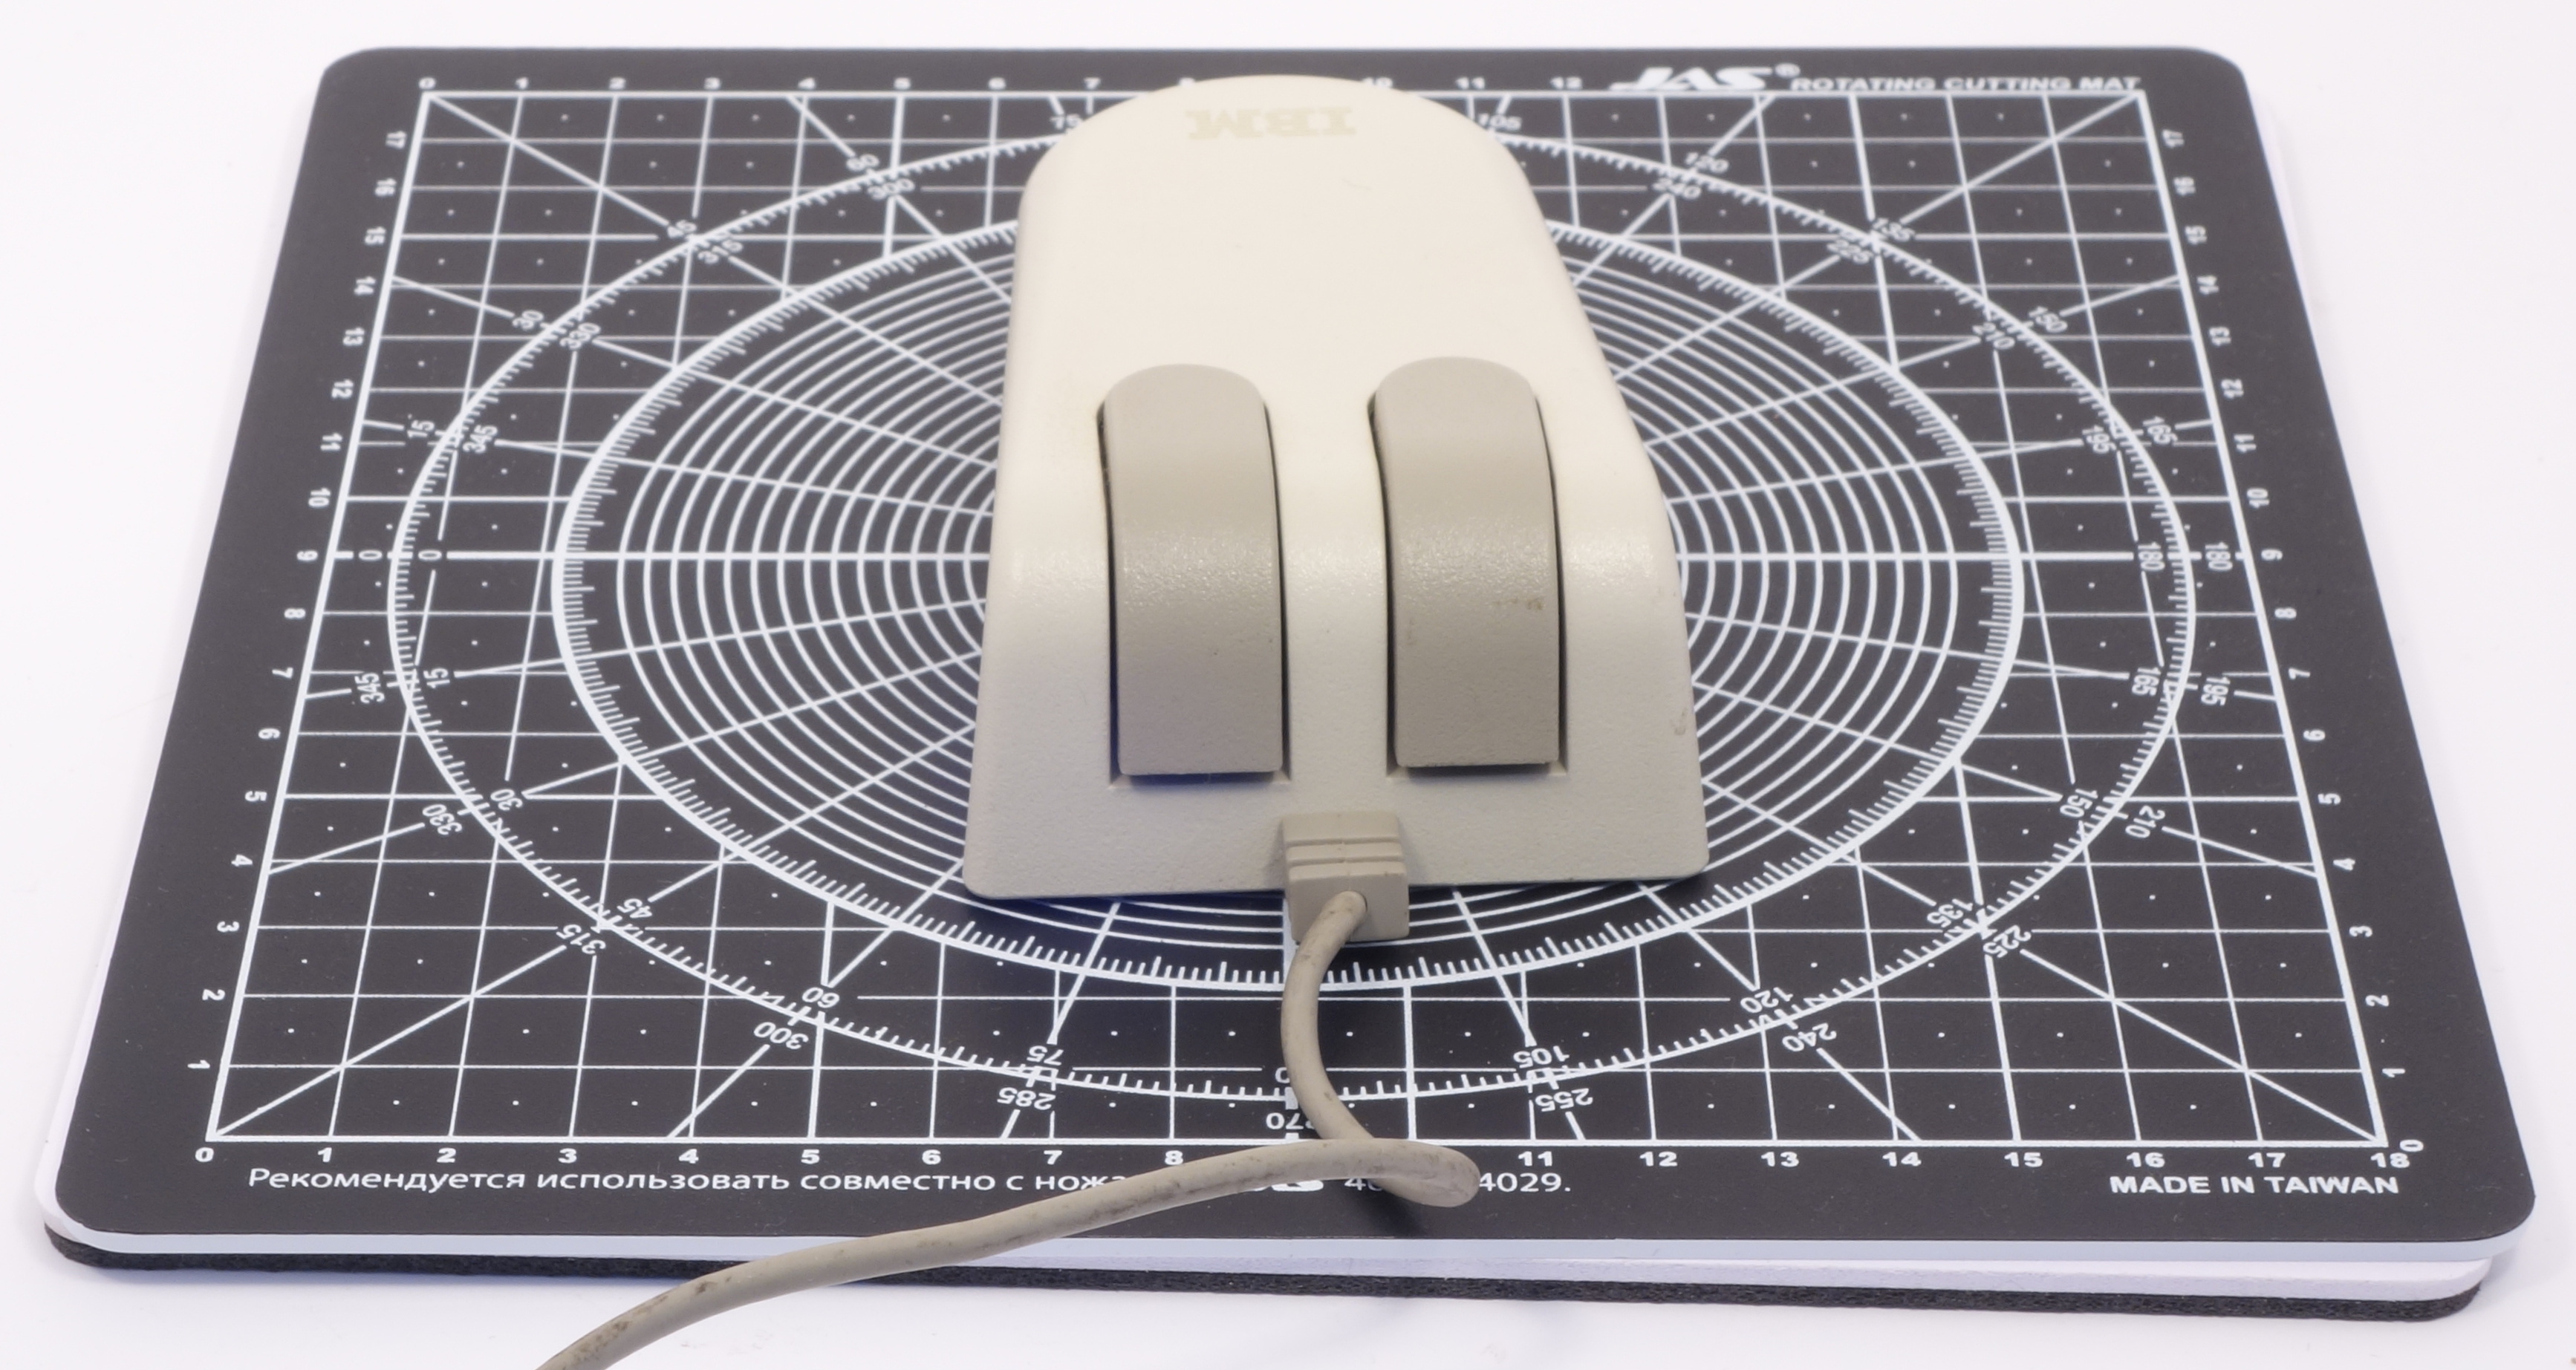
\includegraphics[scale=0.34]{1987_ibm_ps2_mouse/num4.jpg}
    \caption{IBM PS/2 Mouse on a graduated pad with a grid step of 1~cm}
    \label{fig:IBMPS2Size}
\end{figure}

\begin{figure}[h]
    \centering
    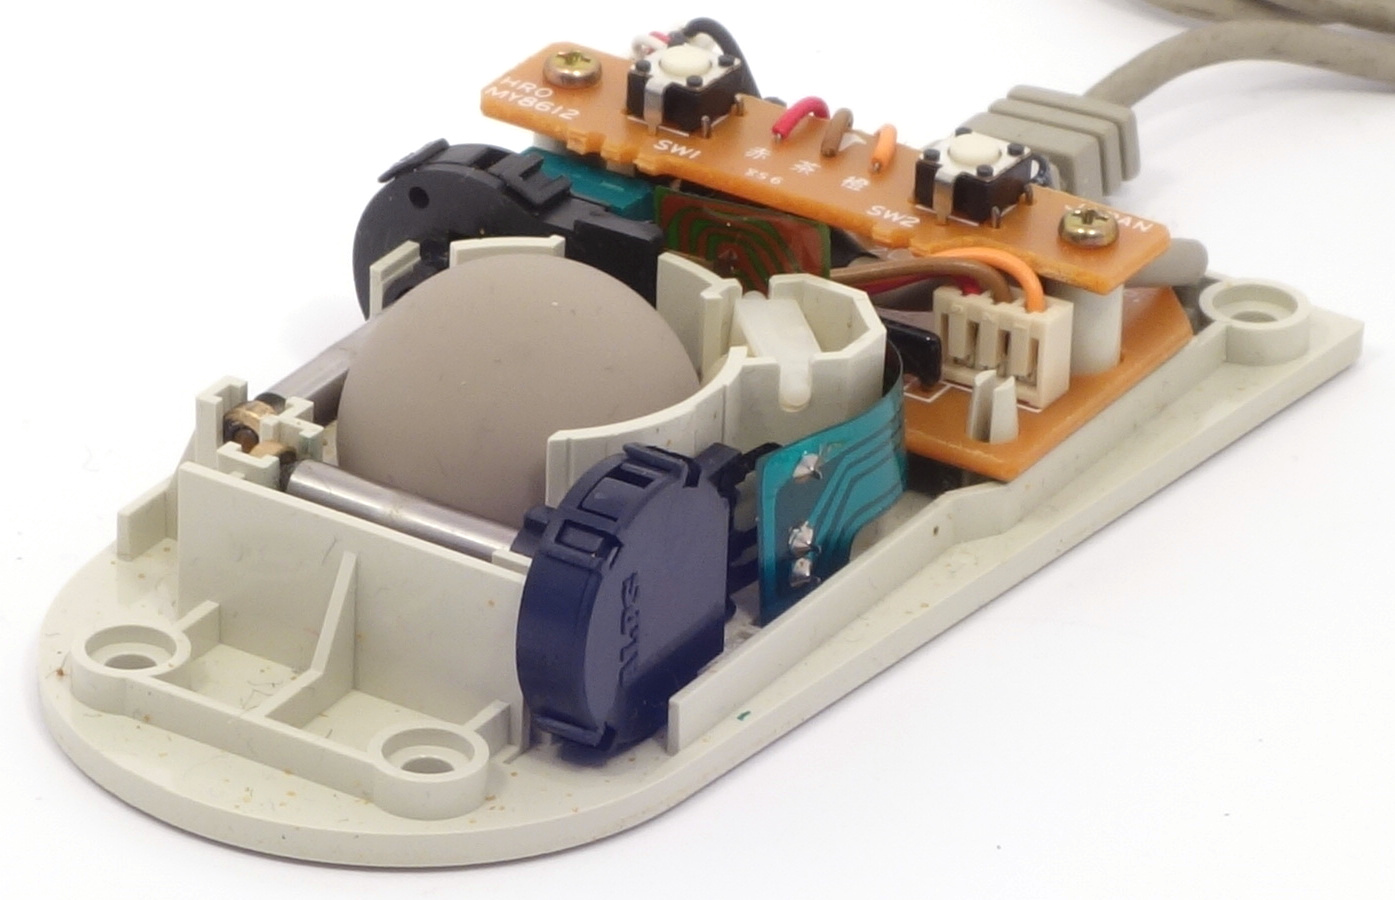
\includegraphics[scale=0.7]{1987_ibm_ps2_mouse/razob1.jpg} 
    \caption{IBM PS/2 Mouse disassembled}
    \label{fig:IBMPS2Inside}
\end{figure}

IBM PS/2 Mouse internals are shown on figure \ref{fig:IBMPS2Inside}. The mouse is a device with a contact encoder made in Japan by Alps. Also, massive metal rollers with bearings should be noted, since they are typical for expensive manipulators.

\end{document}
